\begin{frame}
\begin{block}{cartoon of free cocompletion}
\centering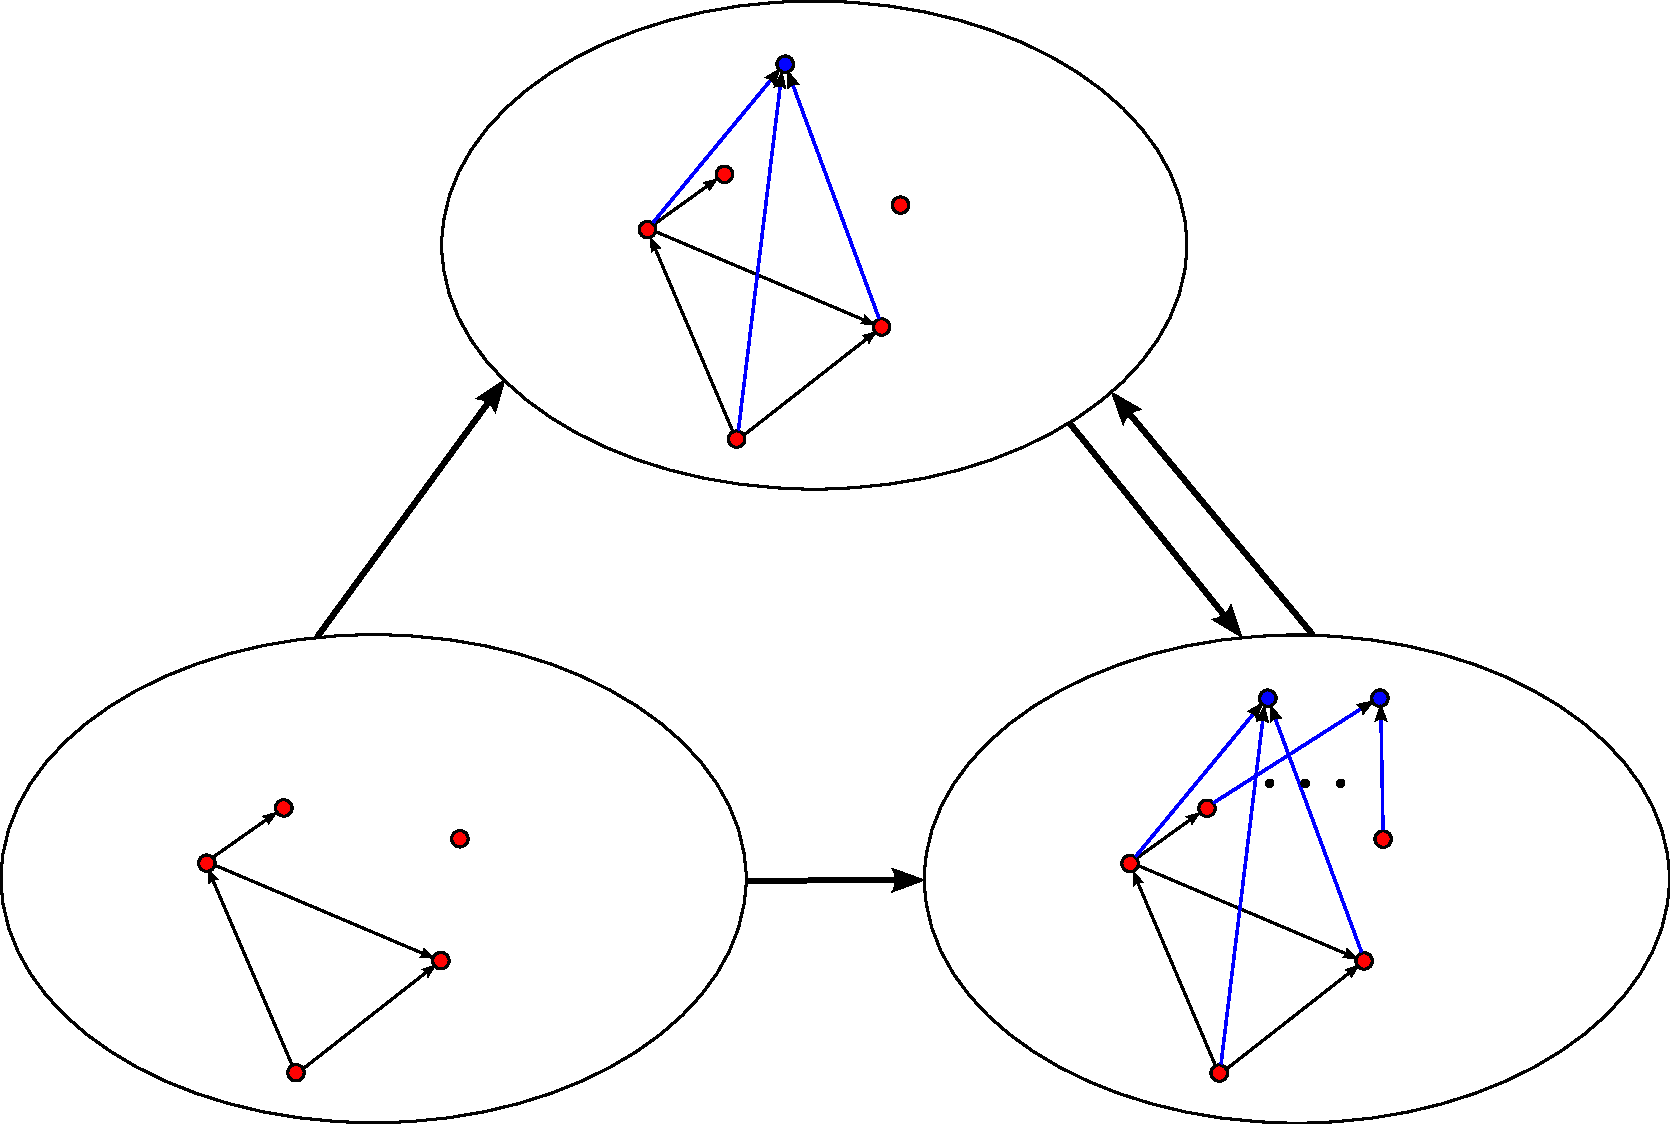
\includegraphics[width=1.0\textwidth]{fig/graphyonedaext.pdf}
\end{block}
%\begin{block}{}
%As a concrete but necessarily incomplete depiction in terms of graphs for intuitive consideration, we can imagine the graph on the left having colimits freely adjoined via Yoneda embedding into the graph on the right (colimits are represented by blue nodes and arrows) and then selecting some of those colimits for inclusion in the category representing {\it global} biological information structures.
%\end{block}
\end{frame}